\documentclass{mini}
\usepackage[utf8]{inputenc}
\usepackage{caption}
\usepackage{subcaption}
\usepackage[polish]{babel}
\usepackage{graphicx}
\usepackage{mathtools}
\usepackage{algpseudocode}
\usepackage{color}
\usepackage{xcolor}
\usepackage{listings}
\usepackage{catchfilebetweentags}
\usepackage{enumitem}

\usepackage{catchfilebetweentags}
\usepackage{etoolbox}
\setcounter{tocdepth}{2}
\makeatletter
\patchcmd{\CatchFBT@Fin@l}{\endlinechar\m@ne}{}
  {}{\typeout{Unsuccessful patch!}}
\makeatother

\addto\extraspolish{%  
 \def\figureautorefname{Rysunek}%  
} 

%------------------------------------------------------------------------------%
\title{Realizacje scenariuszy działań}
\pm{Robert Jakubowski}
\author{Mariusz Ambroziak
\\Paweł Bielicki
\\Karol Bocian
\\Hanna Dziegciar
\\Karol Dzitkowski
\\Mateusz Jankowski
\\Wiktor Ryciuk}
\monthyear{\today}
%------------------------------------------------------------------------------%
\begin{document}
%<*tag>
\section{Przykłady}

\subsection{Pytanie czy dany scenariusz moze wystąpić}

\subsubsection{Historia}

Mick i Sarah są parą, więc mają wspólne produkty spożywcze, ale posiłki zwykle jadają oddzielnie. Pewnego dnia Sarah chce zrobić ciasto, a Mick naleśniki. Nie mogą być one robione w tym samym czasie ze względu konieczność użycia miksera do przygotowania obu. Ponadto, zrobienie jednego lub drugiego dania zużywa cały zapas jajek dostępnych w mieszkaniu, więc trzeba je potem dokupić.

\subsubsection{Opis akcji}

 \textbf{initially}  \textit{eggs}\\
 \textit{(making\_panc,1)}  \textbf{ causes}  \textit{$\neg$ eggs}  \textbf{if}  \textit{eggs}\\
(making\_cake,1)   \textbf{causes} $\neg$ eggs  \textbf{if}  \textit{eggs}\\
 \textbf{impossible}  \textit{\{making\_pan,making\_cake\}}\\
$(buy\_eggs,2)$  \textbf{causes}  \textit{eggs}\\

\subsubsection{Scenariusze}

Sc =$(OBS;ACS)$\\
OBS =  ${\emptyset}$\\
ACS = $((making\_panc;1),0), ((making\_cake,1)2)$\\

Sc2 =$(OBS2;ACS2)$\\
OBS2 = ${\emptyset}$\\
ACS2 =$ ((making\_panc,1),0), ((buy\_eggs,2)2),( (making\_cake,1),4), ((making\_panc,1), 4)$\\


\subsubsection{Kwerendy}

\begin{enumerate}
	\item  \textbf{performing}  \textit{making\_panc}  \textbf{at} $1$  \textbf{when}  \textit{Sc}
	\item  \textbf{performing}  \textit{making\_cake}  \textbf{at} 2  \textbf{when}  \textit{Sc}
	\item  \textbf{ever executable} \textit{Sc}
	\item  \textbf{ever executable} \textit{Sc2}
\end{enumerate}

\subsubsection{Analiza}

Odpowiedzi na kwerendy to odpowiednio:
\begin{enumerate}
	\item \texttt{TRUE},
	\item \texttt{TRUE},
	\item \texttt{TRUE},
	\item \texttt{FALSE},
\end{enumerate}

Zgodnie z diagramem dla scenariuszy  \textit{Sc} i \textit{Sc2}:

\begin{center}
  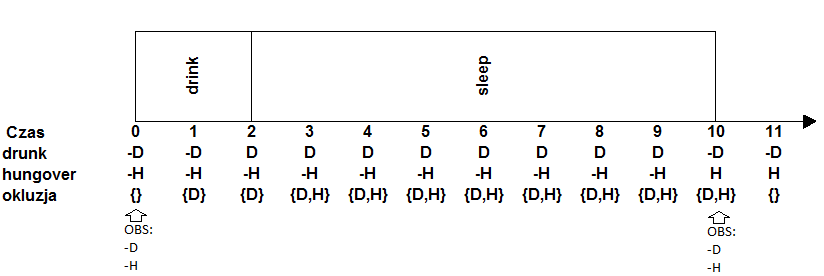
\includegraphics[width=1\textwidth]{Example1}
\end{center}

Scenariusza \textit{ Sc2} nie można wykonać, ponieważ wymaga on jednoczesnego wypełnienia akcji  $\textit{making\_panc}$ i  $\textit{making\_cake}$, co jest niezgodne z warunkami zadania.


\subsection{Pytanie czy dany warunek zachodzi w danym czasie}

\subsubsection{Historia}

Mick i Sarah są parą, więc mają wspólne produkty spożywcze, ale posiłki zwykle jadają oddzielnie. Pewnego dnia Sarah chce zrobić ciasto, a Mick naleśniki. Nie mogą być one robione w tym samym czasie ze względu konieczność użycia miksera do przygotowania obu. Ponadto, zrobienie jednego lub drugiego dania zużywa cały zapas jajek dostępnych w mieszkaniu, więc trzeba je potem dokupić.

\subsubsection{Opis akcji}
 \textbf{initially}  \textit{eggs}\\
$(making\_panc,1)$   \textbf{causes} $\neg$  \textit{eggs} \textbf{ if } \textit{eggs}\\
$(making\_cake,1)$   \textbf{causes} $\neg$  \textit{eggs} \textbf{ if } \textit{eggs}\\
 \textbf{impossible} $\{making\_pan,making\_cake\}$\\
$(buy\_eggs,2)$  \textbf{causes}  \textit{eggs}\\


\subsubsection{Scenariusz}

 \textit{Sc} =$(OBS;ACS)$
 \textit{OBS} =  ${\emptyset}$\\
 \textit{ACS} = $((making\_panc;1),0), ((making\_cake,1)2)$


\subsubsection{Kwerendy}

\begin{enumerate}
	\item  \textit{eggs}  \texttt{at} 1  \textbf{when}  \textit{Sc}
	\item  \textit{eggs} \texttt{ at} 2 \textbf{ when} \textit{ Sc}
\end{enumerate}

\subsubsection{Analiza}

Odpowiedzi na kwerendy to odpowiednio:
\begin{enumerate}
	\item \texttt{TRUE},
	\item \texttt{FALSE}.
\end{enumerate}
	
	Zgodnie z diagramem dla scenariusza \textit{Sc}:

\begin{center}
  
\includegraphics[width=1\textwidth]{Example2}
\end{center}

	Oczywiście warunek akcji \textit{making\_panc} nie jest spełniony w momencie $2$.

\subsection{Pytanie czy dana akcja jest wykonywana w pewnym czasie}

Ten przykład pokazuje przypadek kwerendy, która pyta, czy dana akcja jest wykonywana w pewnym czasie.

\subsubsection{Historia}

Mamy Billa i psa Maxa. Jeśli Bill idzie, to Max biegnie. Jeśli Bill gwiżdże , Max szczeka. Jeśli Bill zatrzymuje się, Max również. Jeśli Bill przestaje gwizdać, to Max przestaje szczekać.

\subsubsection{Opis akcji}

\textbf{initially} $\neg go\_Bill$ \textbf{and} $\neg run\_Max$ \textbf{and} $\neg whistle\_Bill$ \textbf{and} $\neg bark\_Max$ \\
$(goes\_Bill,2)$ \textbf{causes} $run\_Max$\\
$(goes\_Bill,2)$ \textbf{invokes} $(runs\_Max,2)$ \textbf{after} $0$\\
$(runs\_Max,2)$ \textbf{causes} $\neg run\_Max$\\
$(whistles\_Bill,1)$ \textbf{causes} $bark\_Max$\\
$(whistles\_Bill,1)$ \textbf{invokes} $(barks\_Max,1)$ \textbf{after} $0$\\
$(whistles\_Bill,1)$ \textbf{causes} $\neg whistle\_Bill$\\


\subsubsection{Scenariusz}

\textit{Sc} =$(OBS,ACS)$\\
\textit{OBS} = ${\emptyset}$\\
\textit{ACS} = ${ ((goes\_Bill,2),1), ((whistles\_Bill,1),5),((goes\_Bill,2),7)	}$\\

\subsubsection{Kwerendy}

\begin{enumerate}
\item \textbf{performing} $run\_Max$ \textbf{at} $8$ \textbf{when} \textit{Sc}
\item \textbf{performing} $run\_Max$ \textbf{when} \textit{Sc}
\item \textbf{performing} \textbf{at} $8$ \textbf{when} \textit{Sc}
\end{enumerate}

\subsubsection{Analiza}
Odpowiedzi na powyższe kwerendy są następujące:
\begin{enumerate}
\item \texttt{FALSE},
\item \texttt{TRUE},
\item \texttt{TRUE}.
\end{enumerate}
Ilustruje to poniższy diagram:

\begin{center}
  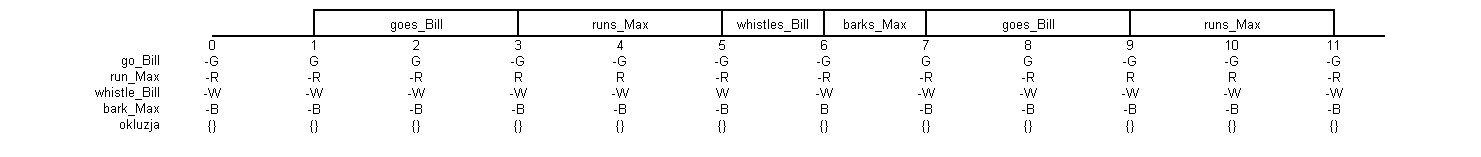
\includegraphics[width=1\textwidth]{Example3}
\end{center}

\subsection{Brak integralności}

Przykład \textit{Brak integralnośći} pokazuje scenariusz, który mimo zgodności z warunkami zadania, jest sprzeczny z logiką \textit{common sense} (z powodu braku warunków integralności).

\subsubsection{Historia}
Mamy Billa oraz komputer. Bill może nacisnąć przycisk \textit{Włącz} lub odłączyć komputer od zasilania. Komputer jest wyłączony i podłączony do zasilania. Jeżeli zostanie naciśnięty jego przycisk \textit{Włącz}, to komputer włącza się.

\subsubsection{Opis akcji}

\textbf{initially} $\neg on\_computer$ \textbf{and} $connect\_power\_computer$ \textbf{and} $\neg swith\_on\_computer$\\
$(clicks\_button\_on,1)$ \textbf{causes} $switch\_on\_computer$\\
$(clicks\_button\_on,1)$ \textbf{invokes} $(switches\_on\_computer,2)$ \textbf{after} $0$\\
$(switches\_on\_computer,1)$ \textbf{causes} $on\_computer$\\
$(disconnects\_power,1)$ \textbf{causes} $on\_computer$ \textbf{and} $\neg swith\_on\_computer$ \\

\subsubsection{Scenariusz}

\textit{Sc} =$(OBS,ACS)$\\
\textit{OBS} = ${\emptyset}$\\
\textit{ACS} = ${ ((clicks\_button\_on,1),1), ((disconnects\_power,1),4),((clicks\_button\_on,1),5)	}$\\

\subsubsection{Kwerendy}

\begin{enumerate}
\item $swith\_on\_computer$ \textbf{at} $6+2$ \textbf{when} \textit{Sc}
\item $swith\_on\_computer$ \textbf{and} $\neg on\_computer$ \textbf{at} $6+2$ \textit{when} \textbf{Sc}
\end{enumerate}


\subsubsection{Analiza}
Powyższy scenariusz jest prawidłowy, lecz zawiera pewną niezgodność. W chwili $t = 4+1$ komputer zostaje odcięty od zasilania. Powinien więc wyłączyć się. Bill chwili $t = 5+1$ naciska przycisk \textit{Włącz}.Komputer zacznie włączać się mimo iż jest odcięty od zasilania. Zachodzą dwa sprzeczne ze sobą stany, tj. $swith\_on\_computer = T$ i $on\_computer=T$. Odpowiedzi na powyższe kwerendy będą odpowiednio: $1.$ \texttt{TRUE} i $2.$ \texttt{FALSE}. Należy zaznaczyć, że odpowiedzi zgodnie ze zdrowym rozsądkiem powinny być sobie równe.

\begin{center}
  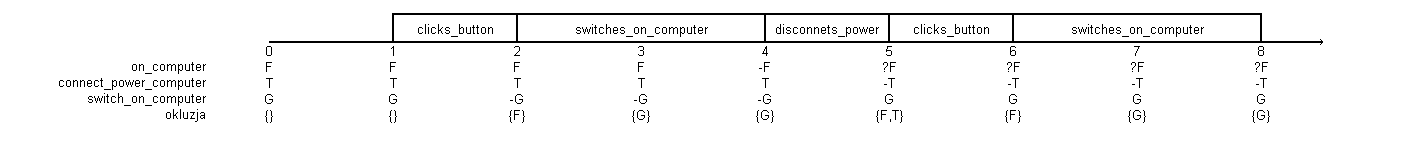
\includegraphics[width=1\textwidth]{Example5}
\end{center}



%</tag>
\end{document}
